\newgeometry{top=2cm,left=2cm,right=2cm,bottom=2cm} 
%
\section{Introduction}
In this thesis, we set out to investigate the properties of the (2+1) dimensional black hole solution, discovered by \textbf{Máximo Bañados}, \textbf{Claudio Teitelboim}, and \textbf{Jorge Zanelli}, known as the \textbf{BTZ black hole}. Our aim is to first discuss the properties of the solution from the perspective of classical general relativity, of which a brief review is located in appendix A. Following that, we aim to investigate the consequences of having the BTZ spacetime be the background of a quantum scalar field theory. As will be shown, the BTZ Green's functions (sometimes referred to as two-point functions) will obey the KMS condition and the black hole will have a non-zero temperature, as is also the case for the Schwarzschild black hole. The structure of the thesis will be as follows:\newline
In \textbf{section 1}, we will first introduce the basic concepts of event horizons and black holes. We will then discuss the properties of some black hole solutions in (3+1) dimensions. Following that, some general features of quantum field theory in curved spaces are discussed. Lastly, we will go over the general features of standard general relativity in (2+1) dimensions.\newline
In \textbf{section 2}, we derive the BTZ metric by solving the \textbf{Einstein Equations} in (2+1) dimensions, assuming the existence of a time-like and a space-like \textbf{Killing vector}. We then discuss how the BTZ spacetime can be obtained by identifying certain points of the 3 dimensional \textbf{anti-de Sitter spacetime}.\newline
In \textbf{section 3}, we investigate the causal structure of the maximally extended static BTZ spacetime. We also discuss the nature of the singularities of the BTZ spacetime, and the existence of \textbf{closed time-like curves} under a specific extension of the spacetime.\newline
In \textbf{section 4}, we first discuss the \textbf{KMS condition} and how it implies that periodicity in imaginary time of the scalar field two-point functions give rise to a non-zero temperature. We then compute the two-point functions on $AdS_3$, and connect them to those of the static BTZ spacetime through the method of images. Lastly, we demonstrate that the static BTZ Green's functions obey the KMS condition, implying a non-zero temperature for the static BTZ black hole.
%
%
%As a final remark, we discuss how the observed temperature can also be obtained by analytic continuation of the static BTZ spacetime.
%
% Not anymore

\subsection{Black hole solutions}
%
The popular idea of a black hole is something all-devouring, something so massive that it is impossible to escape its gravitational pull. A physicists idea of a black hole is not too far from that image, but to give a proper definition of a black hole, we must first define the concept of an event horizon:
%
\theoremstyle{definition}
%
\begin{definition}{\textbf{Event Horizons:}}
The (\textit{future / past}) event horizon of an asymptotically maximally symmetric spacetime, is the boundary of the causal (\textit{past / future}) of conformal infinity $\mathcal{J}$. The causal (\textit{past / future}) of conformal infinity is denoted $J^{\pm}(\mathcal{J})$.
\end{definition}
%
%
\noindent
A \textbf{black hole} is then simply defined as $\mathcal{M} \setminus J^{-}(\mathcal{J})$, where $\mathcal{M}$ is the entire spacetime. This means that any future-directed timelike world line that goes into the black hole is unable to reach null infinity, which is what gives rise to the popular interpretation of black holes that a black hole is something you can not escape.
%
%
\subsubsection{The Schwarzschild Black Hole}
The simplest and most well-known black hole solution is the Schwarzschild black hole in (3+1)-dimensions, with the Schwarzschild metric written in Schwarzschild coordinates as:
%
%
\begin{equation}
ds^2 = -\bigg[1 - \frac{2 \, G \, M}{r} \bigg] \, \mathrm{d}t^2
+ \bigg[1 - \frac{2 \, G \, M}{r} \bigg]^{-1} \, \mathrm{d}r^2
+ r^2 \, \mathrm{d}\Omega_2^2
\end{equation}
%
\begin{equation}
t \in (-\infty, \infty)
\quad , \quad
r \in (0, 2 \, G \, M) \cup (2 \, G \, M, \infty)
\end{equation}
%
%
In the above metric, $d\Omega_2^2$ stands for the metric of a 2-sphere in the usual spherical coordinates. This metric has an apparent singularity at $r = 2 \, G \, M$, but a change of coordinates reveals that it is only a coordinate singularity. The only real singularity is at $r = 0$ where the curvature invariant $R_{\rho\sigma\mu\nu} \,R^{\rho\sigma\mu\nu} $ becomes infinite. One set of coordinates in which this can be seen is the Kruskal–Szekeres coordinates in which the metric takes the form:
%
%
\begin{equation}\label{SW_metric_kruskal}
ds^2 = \frac{32 \, G^3 \, M^3}{r} \, e^{r \, / \, 2 \, G \, M} \,
(-\mathrm{d}T^2 + \mathrm{d}X^2)
+ r^2 \, d\Omega_2^2
%
\quad , \quad
%
T^2 - X^2 < 1
\end{equation}
%
%
In the above $r$ is regarded as an implicit funtion of $X$ and $T$. Switching to these coordinates not only reveals the non-singular nature of the event horizon, it also reveals another curious fact about the spacetime: The traditional Schwarzschild coordinates do not cover the entire spacetime. When switching to Kruskal-Szekeres coordinates, it is possible to follow geodesics to extend the spacetime into a geodesically complete spacetime; a spacetime in which no geodesics stop at finite parameter value. Two diagrams are used to study the causal structure of this maximally extended spacetime; the \textbf{Kruskal diagram} and the \textbf{Conformal diagram}.
%
\begin{figure}[h!]
%
\centering
%
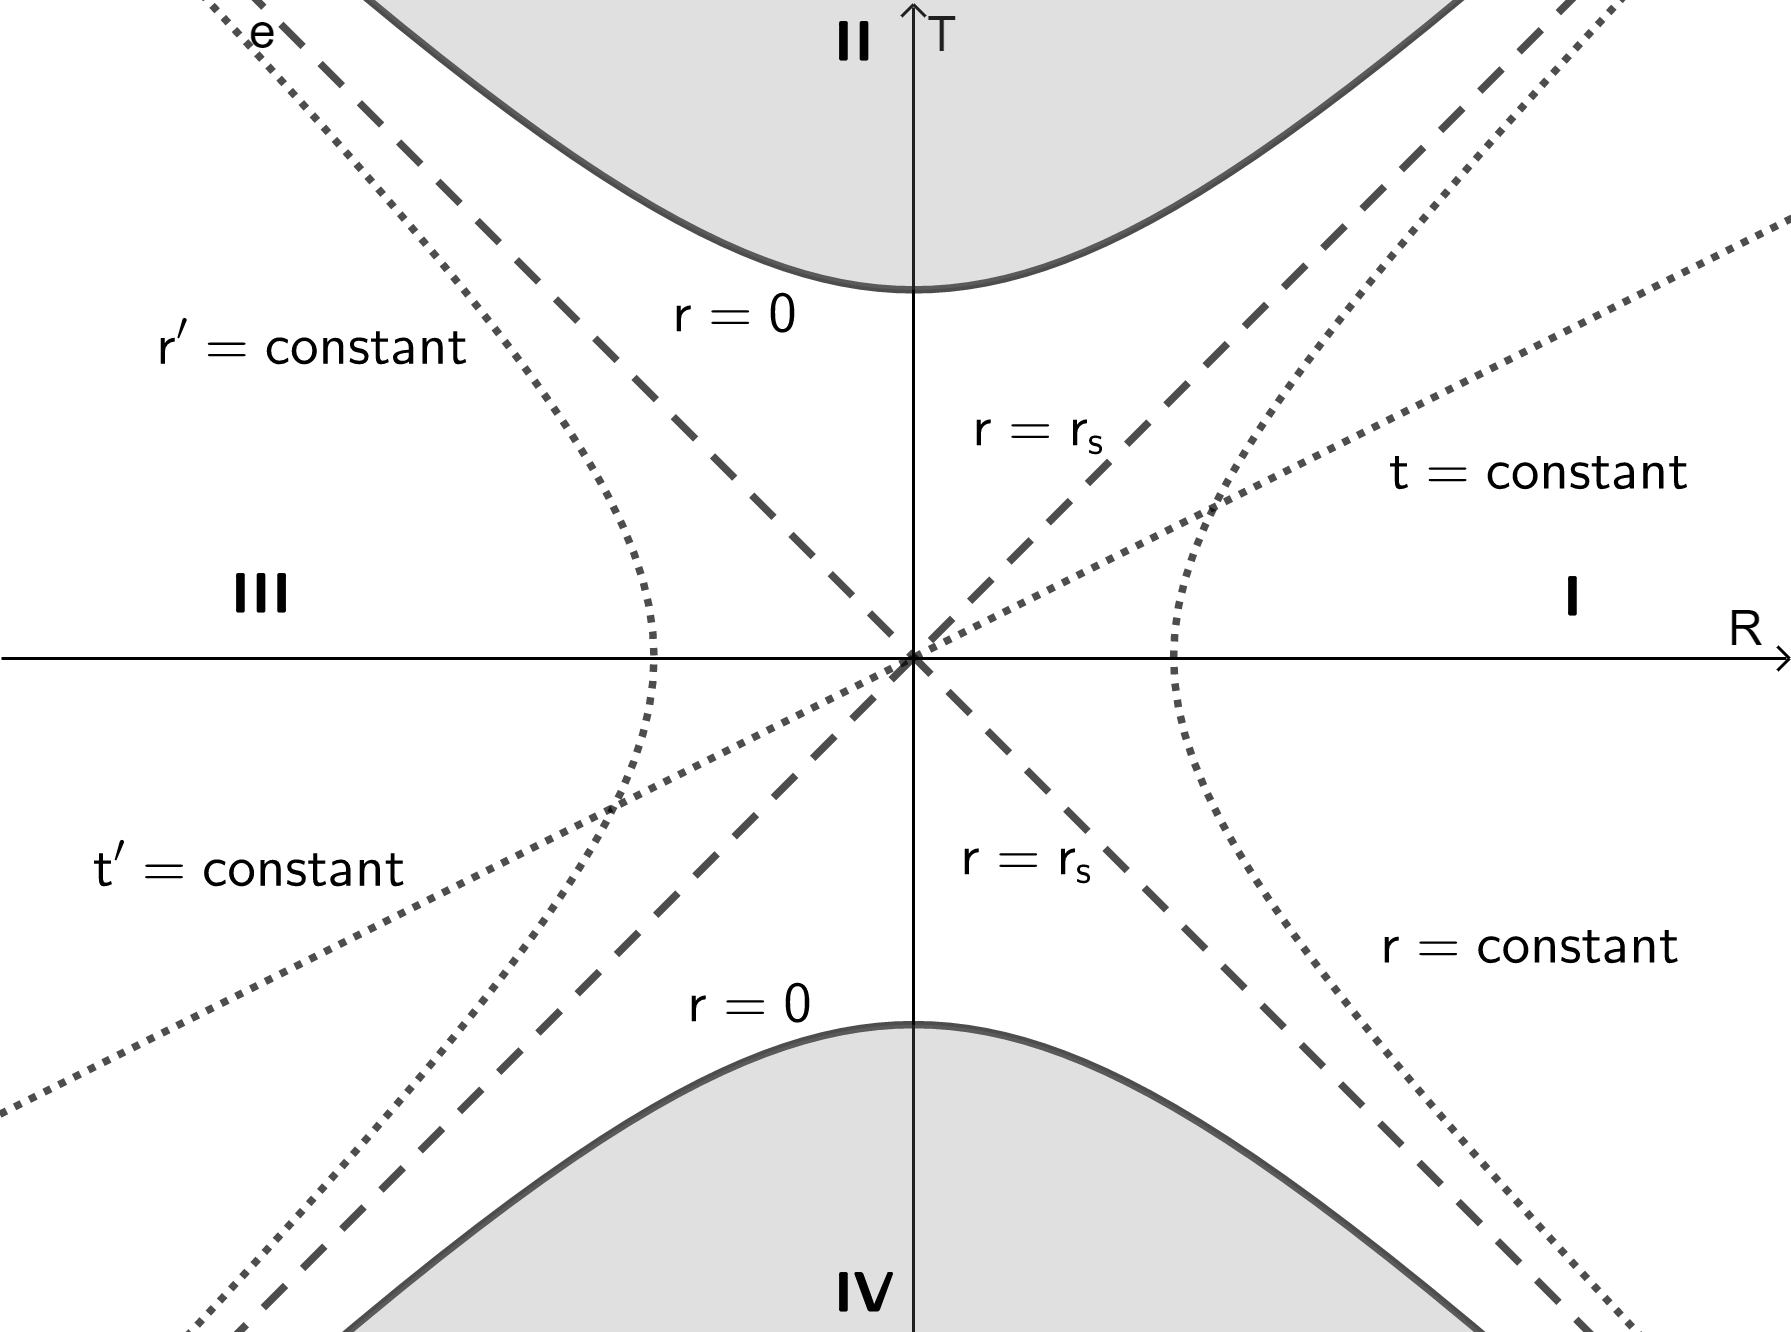
\includegraphics[width=0.69\textwidth]{../pics/Kruskal_Schwarz.png}
%
\caption{Kruskal diagram for the maximally extended Schwarzschild spacetime. The event horizon is located at $r=r_s$, while the curvature singularity is located at $r=0$. The grey areas above and below the $r = 0$ curves are not part of the spacetime.}
%
\label{fig:Kruskal_SW}
%
\end{figure}
%
\newline \noindent
The Kruskal diagram shows the spacetime in the Kruskal-Szekeres coordinates, where light cones stand upright and at $45^{\circ}$ everywhere, as can easily be seen from (\ref{SW_metric_kruskal}). The event horizon at $r = r_s$ naturally seperates the spacetime into four regions. The regions I and III are two disconnected (\textit{meaning not connected by future- or past-directed causal curves}) regions. The region II is the black hole, where hitting the singularity at $r = 0$ is unavoidable following any future-directed timelike path. The most surprising region IV, is called the white hole, and is the time-reversed version of the black hole. This means that all past-directed timelike paths in region IV, must hit the singularity at $r = 0$, or equivalently that it is impossible to enter the white hole from region I or III.\newline \newline
%
%
The Conformal diagram shows the spacetime in a set of compact coordinates, such that the nature of the infinities becomes more apparent. For example, we can easilly see that the structure of the conformal infinities in the regions I and III are identical to that of Minkowski space. We therefore call the Schwarzschild spacetime asymptotically flat. As in the Kruskal diagram, light cones stand upright and at $45^{\circ}$ everywhere in the Conformal diagram.
%
%
\begin{figure}[h!]
%
\centering
%
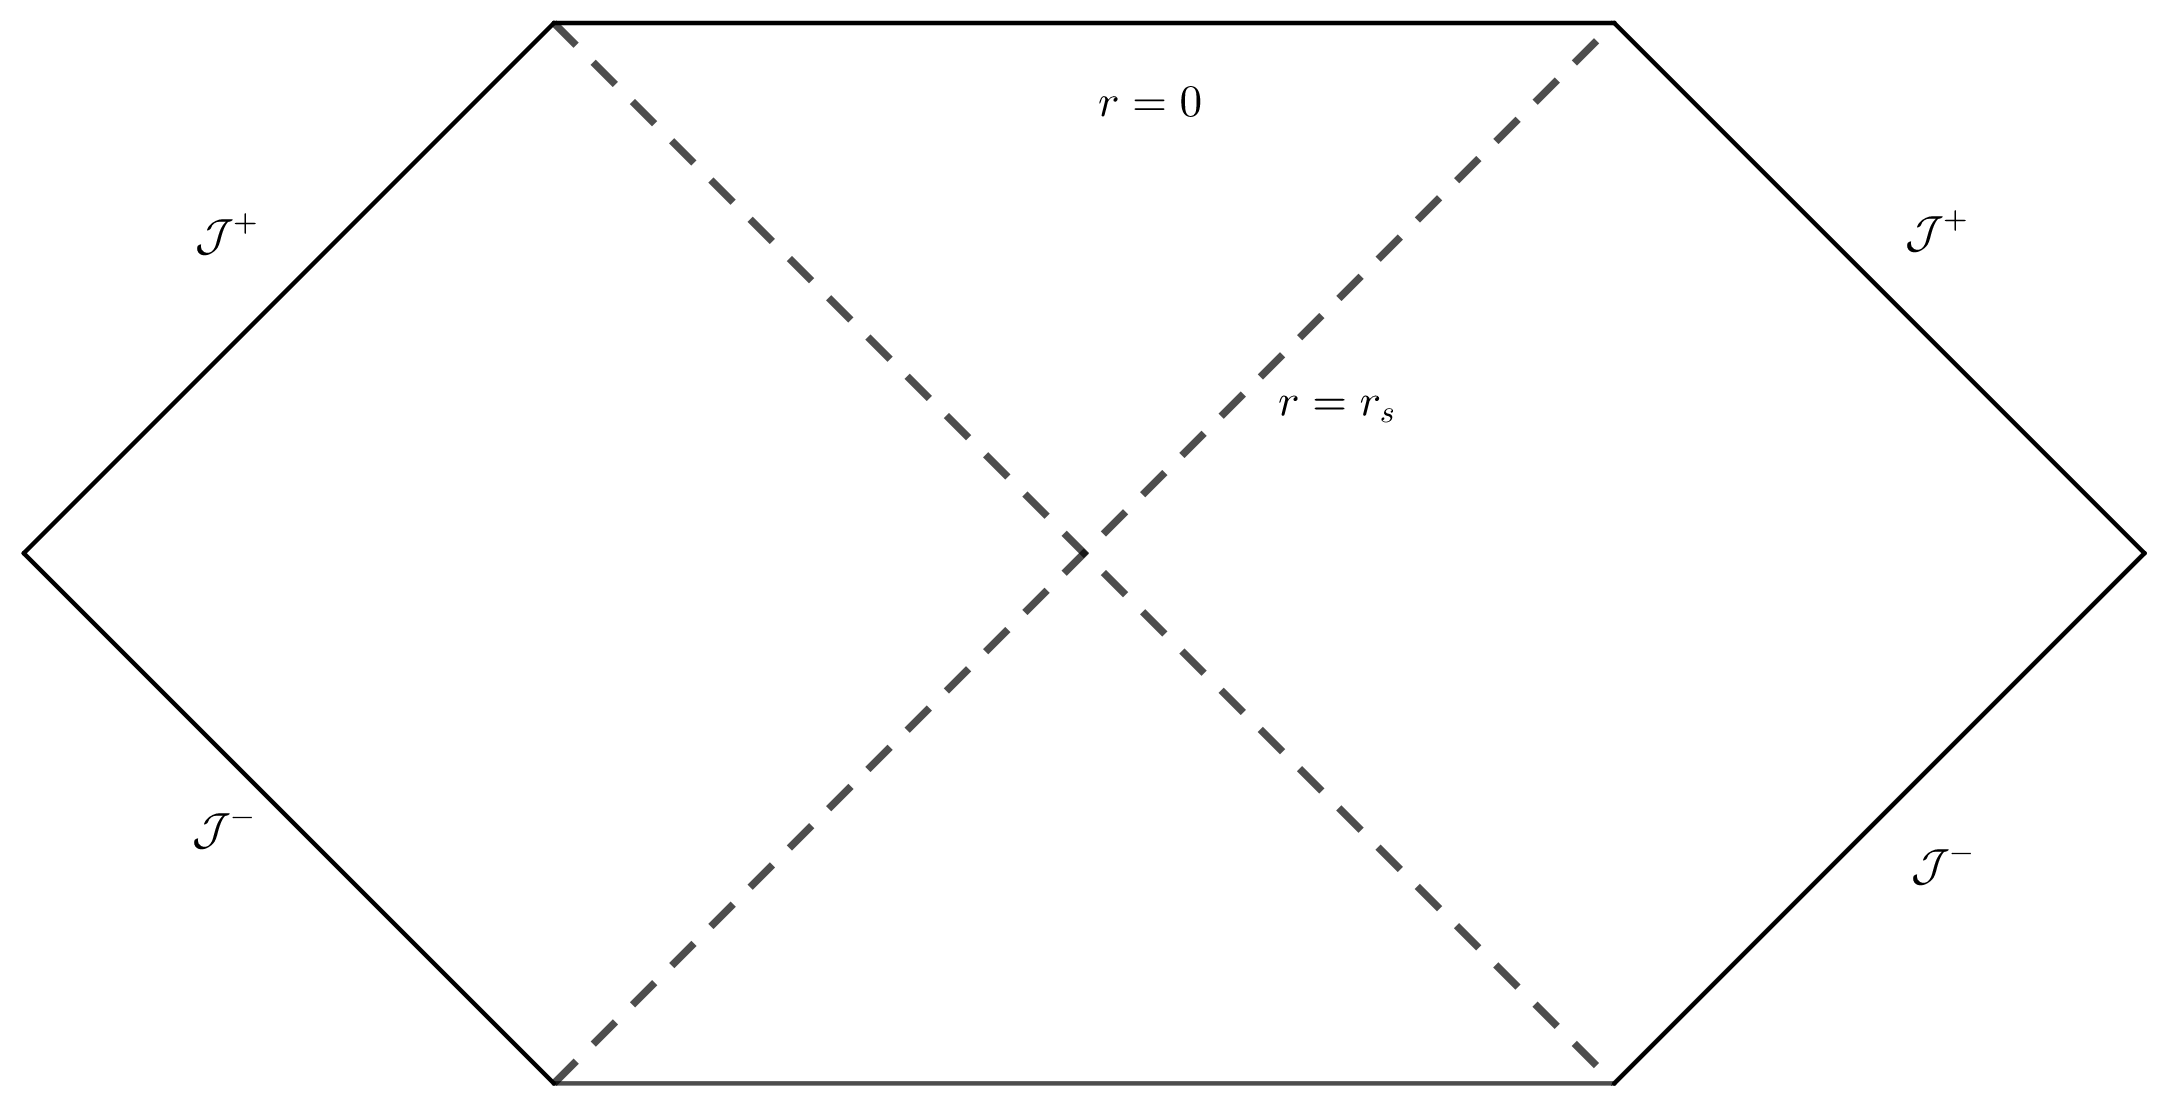
\includegraphics[width=0.86\textwidth]{../pics/SW_stat_Pen.png}
%
\caption{Conformal diagram for the maximally extended Schwarzschild spacetime. The future and past event horizons are located at $r=r_s$, while the curvature singularity is located at $r=0$. Past null infinity $\mathcal{J}^-$ is completely disjoint from future null infinity $\mathcal{J}^+$ in the two asymptotically flat regions.}
%
\label{fig:conformal_SW}
%
\end{figure}
%
%
%

\subsubsection{No-hair Theorem and the Information Paradox}
% Commented out for the time being
%
%%%%%%%%%%%%%%%%%%%%%%%%%%%%%%%%%%%%%%%%%%%%%%%%%%%%%%%%%%%%%%%%%%%%%%%%%%%%%%%%%%%%
%\textit{"Stationary, asymptotically flat black hole solutions to general relativity coupled to electromagnetism that are nonsingular outside the event horizon are fully characterized by the parameters of mass, electric and magnetic charge, and angular momentum."} [Carroll, page 238]\newline \newline
%%%%%%%%%%%%%%%%%%%%%%%%%%%%%%%%%%%%%%%%%%%%%%%%%%%%%%%%%%%%%%%%%%%%%%%%%%%%%%%%%%%%
%
%
Sean Carroll formulates a no-hair theorem in his book \textit{Spacetime and Geometry} in the following way:
%
\theoremstyle{theorem}
%
\begin{theorem}{\textbf{Black holes have no hair:}}
Stationary, asymptotically flat black hole solutions to general relativity coupled to electromagnetism, in 4 or less dimensions, that are nonsingular outside the event horizon, are fully characterized by the parameters of mass, electric and magnetic charge, and angular momentum. \cite{GR} %page 238
\end{theorem}
%
%
\noindent
The essence of this theorem and the reason for its name, is that there are only a small number of properties, parameterizing all black hole solutions. Namely, the mass, charge and spin of the spacetimes. These quantaties can be defined using for example the \textbf{Komar integrals}. This, together with phenomenon of \textbf{Hawking radiation} gives rise to the information paradox, that the information contained in matter seems to be lost when it passes the event horizon of a black hole.


\subsubsection{The Kerr Black Hole}
The Schwarschild Black Hole already discussed is a lot less hairy than what is required by the above no-hair theorem; both its spin and its charge is zero. An example of a Black Hole solution with a non-zero spin would be the \textbf{Kerr Black Hole}, which has a quite intricate metric given in \cite{GR}, which we will state in \textbf{Boyer-Lindquist coordinates} for completion:
%
%
\begin{align}\label{kerr_metric}
ds^2 = & - \left( 1 - \frac{2 \, G \, M \, r}{\rho^2} \right) \mathrm{d}t^2
- \frac{2 \, G \, M \, a \, r \, \sin^2\theta}{\rho^2}
(\mathrm{d}t \, \mathrm{d}\phi + \mathrm{d}\phi \, \mathrm{d}t) \notag\\
& + \frac{\rho^2}{\Delta}\mathrm{d}r^2
+ \rho^2 \, \mathrm{d}\theta^2
+ \frac{\sin^2\theta}{\rho^2} \left[
(r^2 + a^2)^2 - a^2 \Delta \sin^2{\theta}
\right] \mathrm{d}\phi^2
\end{align}
%
\begin{equation}
t \in (-\infty, \infty)
\quad , \quad
r \in (0, r_-) \cup (r_-, r_+) \cup (r_+, \infty)
\quad , \quad
\theta \in (0, \pi)
\quad , \quad
\phi \in (0, 2 \pi)
\end{equation}
%
%
The quantities $\Delta$ and $\rho$ are defined in terms of the coordinates and parameters as follow:
%
%
\begin{equation}
\Delta(r) = r^2 - 2 \, G \, M \, r + a^2
\end{equation}
%
\begin{equation}
\rho^2(r,\theta) = r^2 + a^2 \cos^2{\theta}
\end{equation}
%
%
%%%%%%%%%%%%%%%%%%%%%%%%%%%%%%%%%%%%%%%%%%%%%%%%%%%%%%%%%%%%%%%%%%%%%%%%%%%%%%%%%%%%%%%%
%The Kerr Black Hole has two event horizons: an outer horizon at $r=r_+$, and an inner horizon at $r=r_-$, which makes the causal structure a bit differently from that of the Schwarzschild Black Hole. A particle crossing the outer horizon is \textit{not} forced to pass the ringularity at $\rho = 0$, it is only forced to move towards the ringularity until it crosses the inner horizon. After crossing the inner horizon, the particle is free to move around, and even go through the ringularity, but if it crosses the inner horizon, it will be forced to move away from the ringularity until it crosses the outer horizon again. Furthermore, it will not return to the asymptotically flat region it came from, but rather to a new asymptotically flat region. This means that the area between the outer and inner horizon acts as a black hole (\textit{pulling everything in}), while the area between the inner and outer horizon acts as a black hole (\textit{pushing everything out}). The area past the inner horizon is sometimes called a \textbf{wormhole}. This all becomes more clear when looking at the Conformal diagram for the maximally extended Kerr spacetime.
%%%%%%%%%%%%%%%%%%%%%%%%%%%%%%%%%%%%%%%%%%%%%%%%%%%%%%%%%%%%%%%%%%%%%%%%%%%%%%%%%%%%%%%%
The \textbf{Komar mass} and \textbf{Komar angular momentum} of the Kerr balck hole are respectively $M$ and $M a$. The spacetime posses a curvature singularity at $\rho=0$, corresponding to $r=0$ and $\theta = \frac{\pi}{2}$. Unlike for the Schwarzschild black hole, the singularity is actually a ring and not a point. For this reason, It is referred to as a \textbf{ringularity}. The spacetime has two event horizons, an outer and an inner horizon, corresponding to the two values of $r$ for which $g^{rr} = 0$:
%
%
\begin{equation}
g^{rr}(r) = 0
\quad \Rightarrow \quad
r_{\pm} = G \, M \pm \sqrt{G^2 \, M^2 - a^2}
\end{equation}
%
%
We will later explain this method of identifying event horizons in more detail, when identify the horizons of the BTZ spacetime. In-between the inner and outer horizon, any future directed time-like curve is forced to move in the direction of decreasing $r$. In the region past the inner horizon, any time-like path is free to either go back through the inner horizon or go through the ringularity. The region past the ringularity is the extension of the spacetime to values of $r < 0$. It is sometimes referred to as the \textbf{anti universe}. It can easily be shown that the metric (\ref{kerr_metric}) restricted to curves of $t=const$, $r=const$ and $\theta = \frac{\pi}{2}$, with $r \ll 1$, become:
%
%
\begin{equation}
ds^2 \approx a^2 \, \left( 1 + \frac{2 \, G \, M}{r} \right) \mathrm{d}\phi^2
\end{equation}
%
%
Since $\phi \sim \phi + 2 \pi$, it is clear that for $r < 0$, the curves described above become \textbf{closed time-like curves}. If instead of going through the ringularity, a time-like curve goes back through the inner horizon, it will be forced to move in the direction of decreasing $r$ until it passes the outer horizon. Furthermore, it will not return to the asymptotically flat region it came from, but rather to a new asymptotically flat region. This all becomes more clear when looking at the Conformal diagram for the maximally extended Kerr spacetime:
%
\begin{figure}[h!]
%
\centering
%
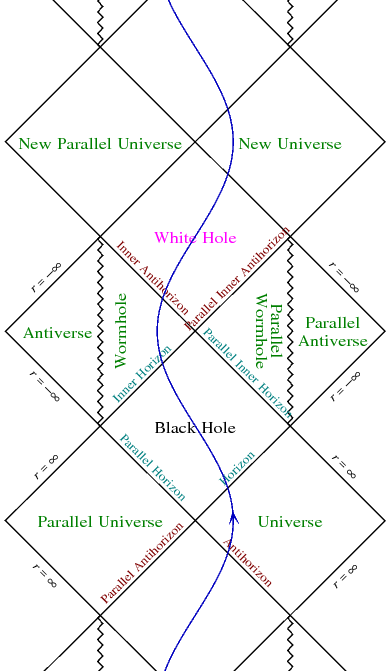
\includegraphics[width=0.38\textwidth]{../pics/penrose_kerr.png}
%
\caption{Conformal diagram for the Kerr spacetime. The blue line is the world line of a particle going through the wormhole. Found at https://jila.colorado.edu/~ajsh/insidebh/penrose.html}
%
\label{fig:conformal_SW}
%
\end{figure}


\subsection{Aspects of QFT on curved backgrounds}
In general curved spacetimes, the exist no notion of \textbf{global inertial coordinates}. As a consequence, there exists no preferred family of spacetime-foliations on which we can define a natural set of basis modes. Different sets of modes will be equally good and although they will exist in the same Hilbert space, they will define different Fock spaces, and specifically different vacuum states. A transformation between to sets of modes $f_i$ and $g_i$ is called a \textbf{Bogoliubov transformation} and given by \cite{GR}
%
%
\begin{equation}
g_i = \sum_j \left( \alpha_{i j} f_j + \beta_{i j} f_j^* \right) \quad , \quad
f_i = \sum_j \left( \alpha^*_{j i} g_j - \beta_{j i} g_j^* \right)
\end{equation}
%
%
The coefficients $\alpha_{i,j}$ and $\beta_{i,j}$ are called the Bogoliubov coefficients and also relate the annihilation and creation operators $\hat{b}_i, \hat{b}_i^{\dagger}$ for $g_i$ and $\hat{a}_i, \hat{a}_i^{\dagger}$ for $f_i$. 
%
%
\begin{equation}
\hat{a}_i = \sum_j \left( \alpha_{j i} \hat{b}_j + \beta_{j i}^* \hat{b}_j^{\dagger} \right) \quad , \quad
\hat{b}_i = \sum_j \left( \alpha^*_{i j} \hat{a}_j - \beta_{i j}^* \hat{a}_j^{\dagger} \right)
\end{equation}
%
%
We use this to calculate the expectation value of the number operator for $g$, $\hat{n}_{g i} = \hat{b}_{i}^{\dagger} \hat{b}_{i}$ in the vacuum state of $f$, $\ket{0_f}$.
%
%
\begin{equation}
\braket{0_f | \hat{n}_{g i} | 0_f} = \sum_{j} \beta_{i j} \beta_{i j}^* 
\end{equation}
%
%
And it now becomes apparent that what is a vacuum state for $f$ is observed in $g$ as a state containing particles.


\subsubsection{The Unruh Effect}
We will now briefly go through the simplest example of this difference in vacuum states, known as the Unruh effect, roughly following the structure of \cite{GR}. The Unruh effect can be stated as \\
\textit{"an accelerating observer in the traditional Minkowski vacuum state will observe a thermal spectrum of particles"} \cite{GR} \\
We start with ordinary (1+1)-dimensional Minkowski space and make the tranformation
%
\begin{equation}
x = \frac{1}{a} \, e^{a \xi} \, \sinh(a \eta) \quad, \quad
t = \frac{1}{a} \, e^{a \xi} \, \cosh(a \eta)
\end{equation}
%
We call the coordinates $(\xi, \eta)$ the \textbf{Rindler coordinates}. It can be shown that they cover the patch I given by $x>|t|$ known as \textbf{Rindler space} and that the we can cover the patch IV given by $x<|t|$ by simply adding a minus sign on each coordinate. In Rindler coordinates, curves of constant acceleration are given by
\begin{equation}
\eta(\tau) = \frac{\alpha}{a} \tau \quad, \quad
\xi(\tau) = \frac{1}{a} \ln \left( \frac{a}{\alpha} \right)
\end{equation}
and the metric takes the form
\begin{equation}
\mathrm{d}s^2 = e^{2 \alpha \xi} (- \mathrm{d} \eta^2 + \mathrm{d} \xi^2 )
\end{equation}
%
%
\begin{figure}[h!]
%
\centering
%
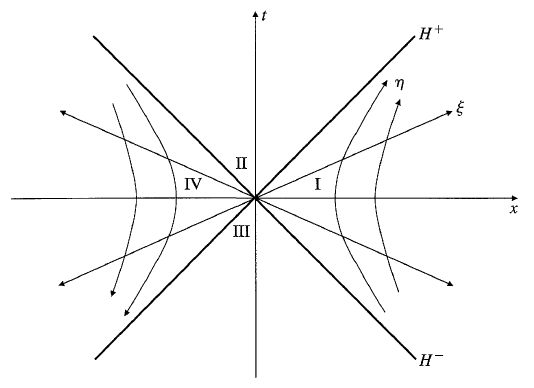
\includegraphics[width=0.8\textwidth]{../pics/Rindler_space.png}
%
\caption{A picture of flat space in Rindler coordinates. $H^+$ and $H^-$ are killing horizons of $\partial_{\eta}$. Found in \cite{GR}}
%
\end{figure}
%
%
Solving the Klein-Gordon equation $\Box \, \phi = 0$ in Rindler coordinates gives us plane waves, but because the future directed Killing vector is $\partial_{\eta}$ and $-\partial_{\eta}$ in patch I and IV respectively, we have a difference in sign for the positive frequency plane wave in the two regions, leading us to define two different plane wave solutions:
\begin{equation}
g_k^{(1)} = 
\begin{cases}
\frac{1}{\sqrt{4 \pi \omega}} e^{-i \omega \eta + i k \xi} & \text{I} \\
0 & \text{IV}
\end{cases}
\end{equation}
\begin{equation}
g_k^{(2)} = 
\begin{cases}
0 & \text{I} \\
\frac{1}{\sqrt{4 \pi \omega}} e^{i \omega \eta + i k \xi} & \text{IV}
\end{cases} \; \;
\end{equation}
We now have two different but equally good sets of modes in Rindler and Minkowski coordinates. We could in theory calculate the Bogoliubov coefficients for these modes and use that to evaluate the expectation value of the number operator for the Rindler coordinates in the Minkowski vacuum. However such a calculation would be long and cumbersome. In \cite{GR} this calculation has been made easier by introducing a set of modes that share the vacuum state with Minkowski but is simpler connected to the Rindler modes. We will not go through his calculation, but state his result:
\begin{equation}
\braket{0_M | \hat{n}_R^{(1)}(k) | 0_M} = \frac{1}{e^{2 \omega \pi / a} - 1} \delta(0)
\end{equation}
which is a thermal spectrum at the temp $T = \frac{a}{2 \pi}$. This is exactly the Unruh effect. A static observer at the event horizon of a Schwarzschild black hole will feel the gravitational pull of the black hole and therefore must be accelerated in order to stay at constant $r$. This leads \cite{GR} to explain Hawking Radiation in terms of the Unruh effect by noting that the spacetime is locally flat at the event horizon. This argument seems to hold for objects much less exotic than black holes though, since any static observer close to a gravitational body must accelerate to remain at a fixed distance to that body. A more convincing way to show that we can associate a temperature with the black hole is to show that its \textbf{Green's Function} has all the properties of a thermal Green's Function. We will show this explicitly in (2+1) dimensions, where Einstein gravity has some special properties.

%For that reason, we will instead argue for the Hawking Radiation by showing that the \textbf{Green's Function} for the BTZ black hole is periodic.



\subsection{Gravity in (2+1) dimensions}
One very important feature of standard Einstein gravity in (2+1) dimensions, is the fact that vacuum solutions have no local degrees of freedom. Said another way, all vacuum solutions to the \textbf{Einstein Equations} in (2+1) dimensions are locally isomorphic to one of the three maximally symmetric spaces; de Sitter space, ant-de Sitter space or Minkowski space. We will now show that this is indeed the case. Using the traces of the \textbf{Riemann tensor}; the \textbf{Ricci tensor} and \textbf{Ricci scalar}, we define a new tensor $C_{\rho\sigma\mu\nu}$, called the \textbf{Weyl tensor}. This tensor is defined by:
%
%
\begin{equation}\label{1.1}
C_{\rho\sigma\mu\nu} = R_{\rho\sigma\mu\nu}
- \frac{2}{(n-2)} \, (g_{\rho[\mu} \, R_{\nu]\sigma} - g_{\sigma[\mu} \, R_{\nu]\rho})
+ \frac{2}{(n-1) \, (n-2)} \, g_{\rho[\mu} \, g_{\nu]\sigma} \, R
\end{equation}
%
%
The Weyl tensor possesses the same symmetries as the Riemann tensor, and satisfies the condition:
%
%
\begin{equation}\label{1.2}
{C^{\rho}}_{\sigma\rho\nu} = 0
\end{equation}
%
%
Because the Weyl tensor and the Riemann tensor have the samme symmetries, the LHS of (\ref{1.2}) will be a symmetric tensor. It can be shown that the number of independent components of the Riemann tensor $D_{Riem}$, on an $n$-dimensional manifold is given by:
%
%
\begin{equation}
D_{Riem} = \frac{n^2 \, (n^2 - 1)}{12}
\end{equation}
%
%
The number of independent components of a symmetric $(0,2)$-tensor $D_{sym}$, on an $n$-dimensional manifold is of cause given by:
%
%
\begin{equation}
D_{sym} = \frac{n \, (n + 1)}{2}
\end{equation}
%
%
Thus, the number of independent components of the Wyel tensor $D_{Weyl}$, on an $n$-dimensional manifold will be given by:
%
%
\begin{equation}
D_{Weyl} = D_{Riem} - D_{sym} = \frac{n^2 \, (n^2 - 1)}{12} - \frac{n \, (n + 1)}{2}
\end{equation}
We see that for $n=3$, we have $D_{Weyl} = 0$. Thus, in a $3$-dimensional spacetime, we can use (\ref{1.1}) to express the Riemann tensor in terms of its traces:
%
%
\begin{equation}
R_{\rho\sigma\mu\nu} =
2 \, (g_{\rho[\mu} \, R_{\nu]\sigma} - g_{\sigma[\mu} \, R_{\nu]\rho})
- g_{\rho[\mu} \, g_{\nu]\sigma} \, R
\end{equation}
%
%
Now we look at the \textbf{Einstein Equations} in vacuum with a cosmological constant $\Lambda$:
%
%
\begin{equation}\label{1.7}
R_{\mu\nu} - \frac{1}{2} \, R \, g_{\mu\nu} + \Lambda \, g_{\mu\nu} = 0
\end{equation}
%
%
Taking the trace of (\ref{1.7}) we obtain, on a $3$-dimensional spacetime, the relation:
%
%
\begin{equation}\label{1.8}
R = 6 \, \Lambda
\end{equation}
%
%
If we now substitute (\ref{1.8}) back into (\ref{1.7}), we obtain the equation:
%
%
\begin{equation}
R_{\mu\nu} = 2 \, \Lambda \, g_{\mu\nu}
\end{equation}
%
%
Thus, for a metric on a $3$-dimensional spacetime, satisfying (\ref{1.7}), the Riemann tensor takes the form:
%
%
\begin{equation}
\boxed{
R_{\rho\sigma\mu\nu} =
\Lambda \, (g_{\rho\mu} \, g_{\nu\sigma} - g_{\rho\nu} \, g_{\mu\sigma})
}
\end{equation}
%
%
We now see that any solution to the Einstein equations, on a $3$-dimensional spacetime, will locally be isomorphic to a \textbf{maximally symmetric} space (\textit{$dS_3$, $AdS_3$ or $M_3$, depending on the sign of $\Lambda$}).

%%%%%%%%%%%%%%%%%%%%%%%%%%%%%%%%%%%%%%%%%%%%%%%%%%%%%%%%%%%%%%%%%%%%%%%%%%%%%%%%%%%%%%%
%From (\ref{1.8}), we also see that the \textbf{Einstein-Hilbert action}:
%%
%%
%\begin{equation}
%I_{EH} = \frac{1}{16 \, \pi \, G} \, \int_{\mathcal{M}} d^3x \, \sqrt{-g}  \, (R - 2 \, \Lambda)
%\end{equation}
%%
%%
%Will in general be infinte, for non-compact spacetime manifolds $\mathcal{M}$. Therefore, a boundary term is usually added to the Einstein-Hilbert action, such that the total action becomes:
%%
%%
%\begin{equation}
%I = \frac{1}{16 \, \pi \, G} \, \bigg[ 
%\int_{\mathcal{M}} d^3x \, \sqrt{-g}  \, (R - 2 \, \Lambda)
%+ \int_{\partial \mathcal{M}} d^2x \, \sqrt{-h} \, K
%\bigg]
%\end{equation}
%%
%%
%Where $h_{ij}$ is the induced metric on $\partial \mathrm{M}$, and $K_{ij}$ is the extrinsic curvature on $\partial \mathrm{M}$.
%%%%%%%%%%%%%%%%%%%%%%%%%%%%%%%%%%%%%%%%%%%%%%%%%%%%%%%%%%%%%%%%%%%%%%%%%%%%%%%%%%%%%%%
